This chapter describes the process of desigining the molecule chip experiment.
This was motivated by three main factors: the need to integrate with the
existing experiment, the core proposal of confining molecules close to a
microwave guide, and the practicalities of fabricating the chip.
%
Each of these factors will be addressed in order. We begin with a discussion of
the existing experiment, and where the chip fits into it. We will see that this
lead us to the conclusion that magnetic traps would be most suitable for our
experiment. Trapping close to the microwave guides requires bringing the
molecules close to the surface of the trap, a loading procedure that was
thorourghly investigated with simulations, and analysis of the phase-space
acceptance of the traps. Problems arising from fabrication will mainly be
discussed in the following chapter.

\section{Experiment overview}

Our ultracold molecules are created using the methods described above, with our
apparatus, including the proposed chip chamber shown in
\myfigref{design:fig:vacuumsystem}. A buffer-gas source is used to create
\CaF{} molecules in the source chamber, with the beam being longitudinally and
transversely slowed before it is captured in a MOT inside the collisions
chamber.

\begin{figure}[htb]
  \centering
  \includegraphics[width=0.7\textwidth]{figs/experiment_placeholder.png}
  \caption{
    \cm{To be replaced with a proper CAD drawing of the experiment}
    A top-down view of the planned \CaF{} experiment is shown. Molecules are
    created in the source chamber in a buffer-gas cell. They are then
    laser-slowed  and undergo transverse
    cooling, before being captured in the collisions chamber.
    Here we can cool the
    molecules using the methods described in and perform
    experiments in collisions. All these are explained further in \cm{theory
    chapter} and \inlinerefs{Jurgilas2021, JurgilasIOP2021,
    PhysRevLett.126.153401}. The magnetic transport
    trap (MTT) can transfer a cloud of molecules to the neighbouring tweezer
    chamber (for the optical tweezer experiment). The chip chamber will be
    positioned next to the tweezer chamber, and will receive molecules from the
    MTT in the same way. Inset, an exploded view of the flange assembly. The
    chip is mounted on a PCB for current (and later microwave) delivery. This
    is positioned above a large copper U-wire for intermediary trapping of
    molecules. The U-wire is electrically isolated by aluminium nitride
    plates.}
  \label{design:fig:vacuumsystem}
\end{figure}

The \CaF{} MOT is the workhorse of our experiment, providing molecules which
can be further cooled cooled further (as discussed above) used for experiments
in collisions with \Rb{} atoms (see \inlinerefs{Jurgilas2021, JurgilasIOP2021,
PhysRevLett.126.153401}) and optical tweezers. The tweezer experiment is
undertaken in the neighbouring tweezer chamber, which is loaded by transporting
molecules in a magnetic transport trap (MTT), a quadrupole trap with coils
mounted on a transport stage outside the vacuum chamber. This transport of the
molecules is similar to that used in
\inlinerefs{Lewandowski2003,PhysRevResearch.1.033035} and elsewhere, it will be
discussed further below and in \cm{transport chapter}.

The chip experiment will integrate into this setup as shown in
\myfigref{design:fig:vacuumsystem}, an additional chamber will be mounted
further downstream of the transport stage, so that molecules can be brought
straight through the tweezer chamber from the collisions chamber.  Since the
molecules will be brought into the chamber inside magnetic trap, we propose to
transfer them gradually into other magnetic traps formed on the chip.
%
Not only does this take advantage of the known, long-lived \CaF{} states in the
trap~\cite{WilliamsMagnetic2018}, but it allows us to follow the well-trodden
path of magnetic trapping near a chip, as has been outlined in previous
chapters.  The transfer to the chip will take the molecules through a series of
magnetic traps of decreasing size until they are in the smallest trap, similar
to what has previously been done in atom chips \cite{Reichel1999} or for
guiding molecules near surfaces \cite{Meek2009}

The chip will be held in its chamber recessed in a PCB used for power (and
later microwave) delivery. We use an aluminium-core PCB to ensure good heat
conduction away from the chip and we refer to it as the subchip.  This is
attached to a large copper heatsink, which has a large U-wire built into it,
isolated from the rest of the copper by aluminium-nitride plates. The heatsink
connects to a flange equipped with a \cm{?} pin feedthrough for chip currents,
and two high-current feedthroughs to power the U-wire.

% TODO Ensure I go on to discuss the current drivers
% TODO confirm distance in this para
We refer to this entire device as the flange assembly, and it is shown in the
inset of \myfigref{design:fig:vacuumsystem} and in
\mysubfigref{design:fig:chipexperiment} It will be mounted so that the chip is
\SI{3}{\milli\meter} away from the transport axis and facing the floor,
allowing us to trap and then drop the molecules for imaging.  External magnetic
coils will provide the bias fields, and currents will be provided by drivers
discussed in \cm{a later chapter.} {a}.

\begin{figure}[ht]
  \centering
  \begin{subfigure}[b]{0.45\textwidth}
    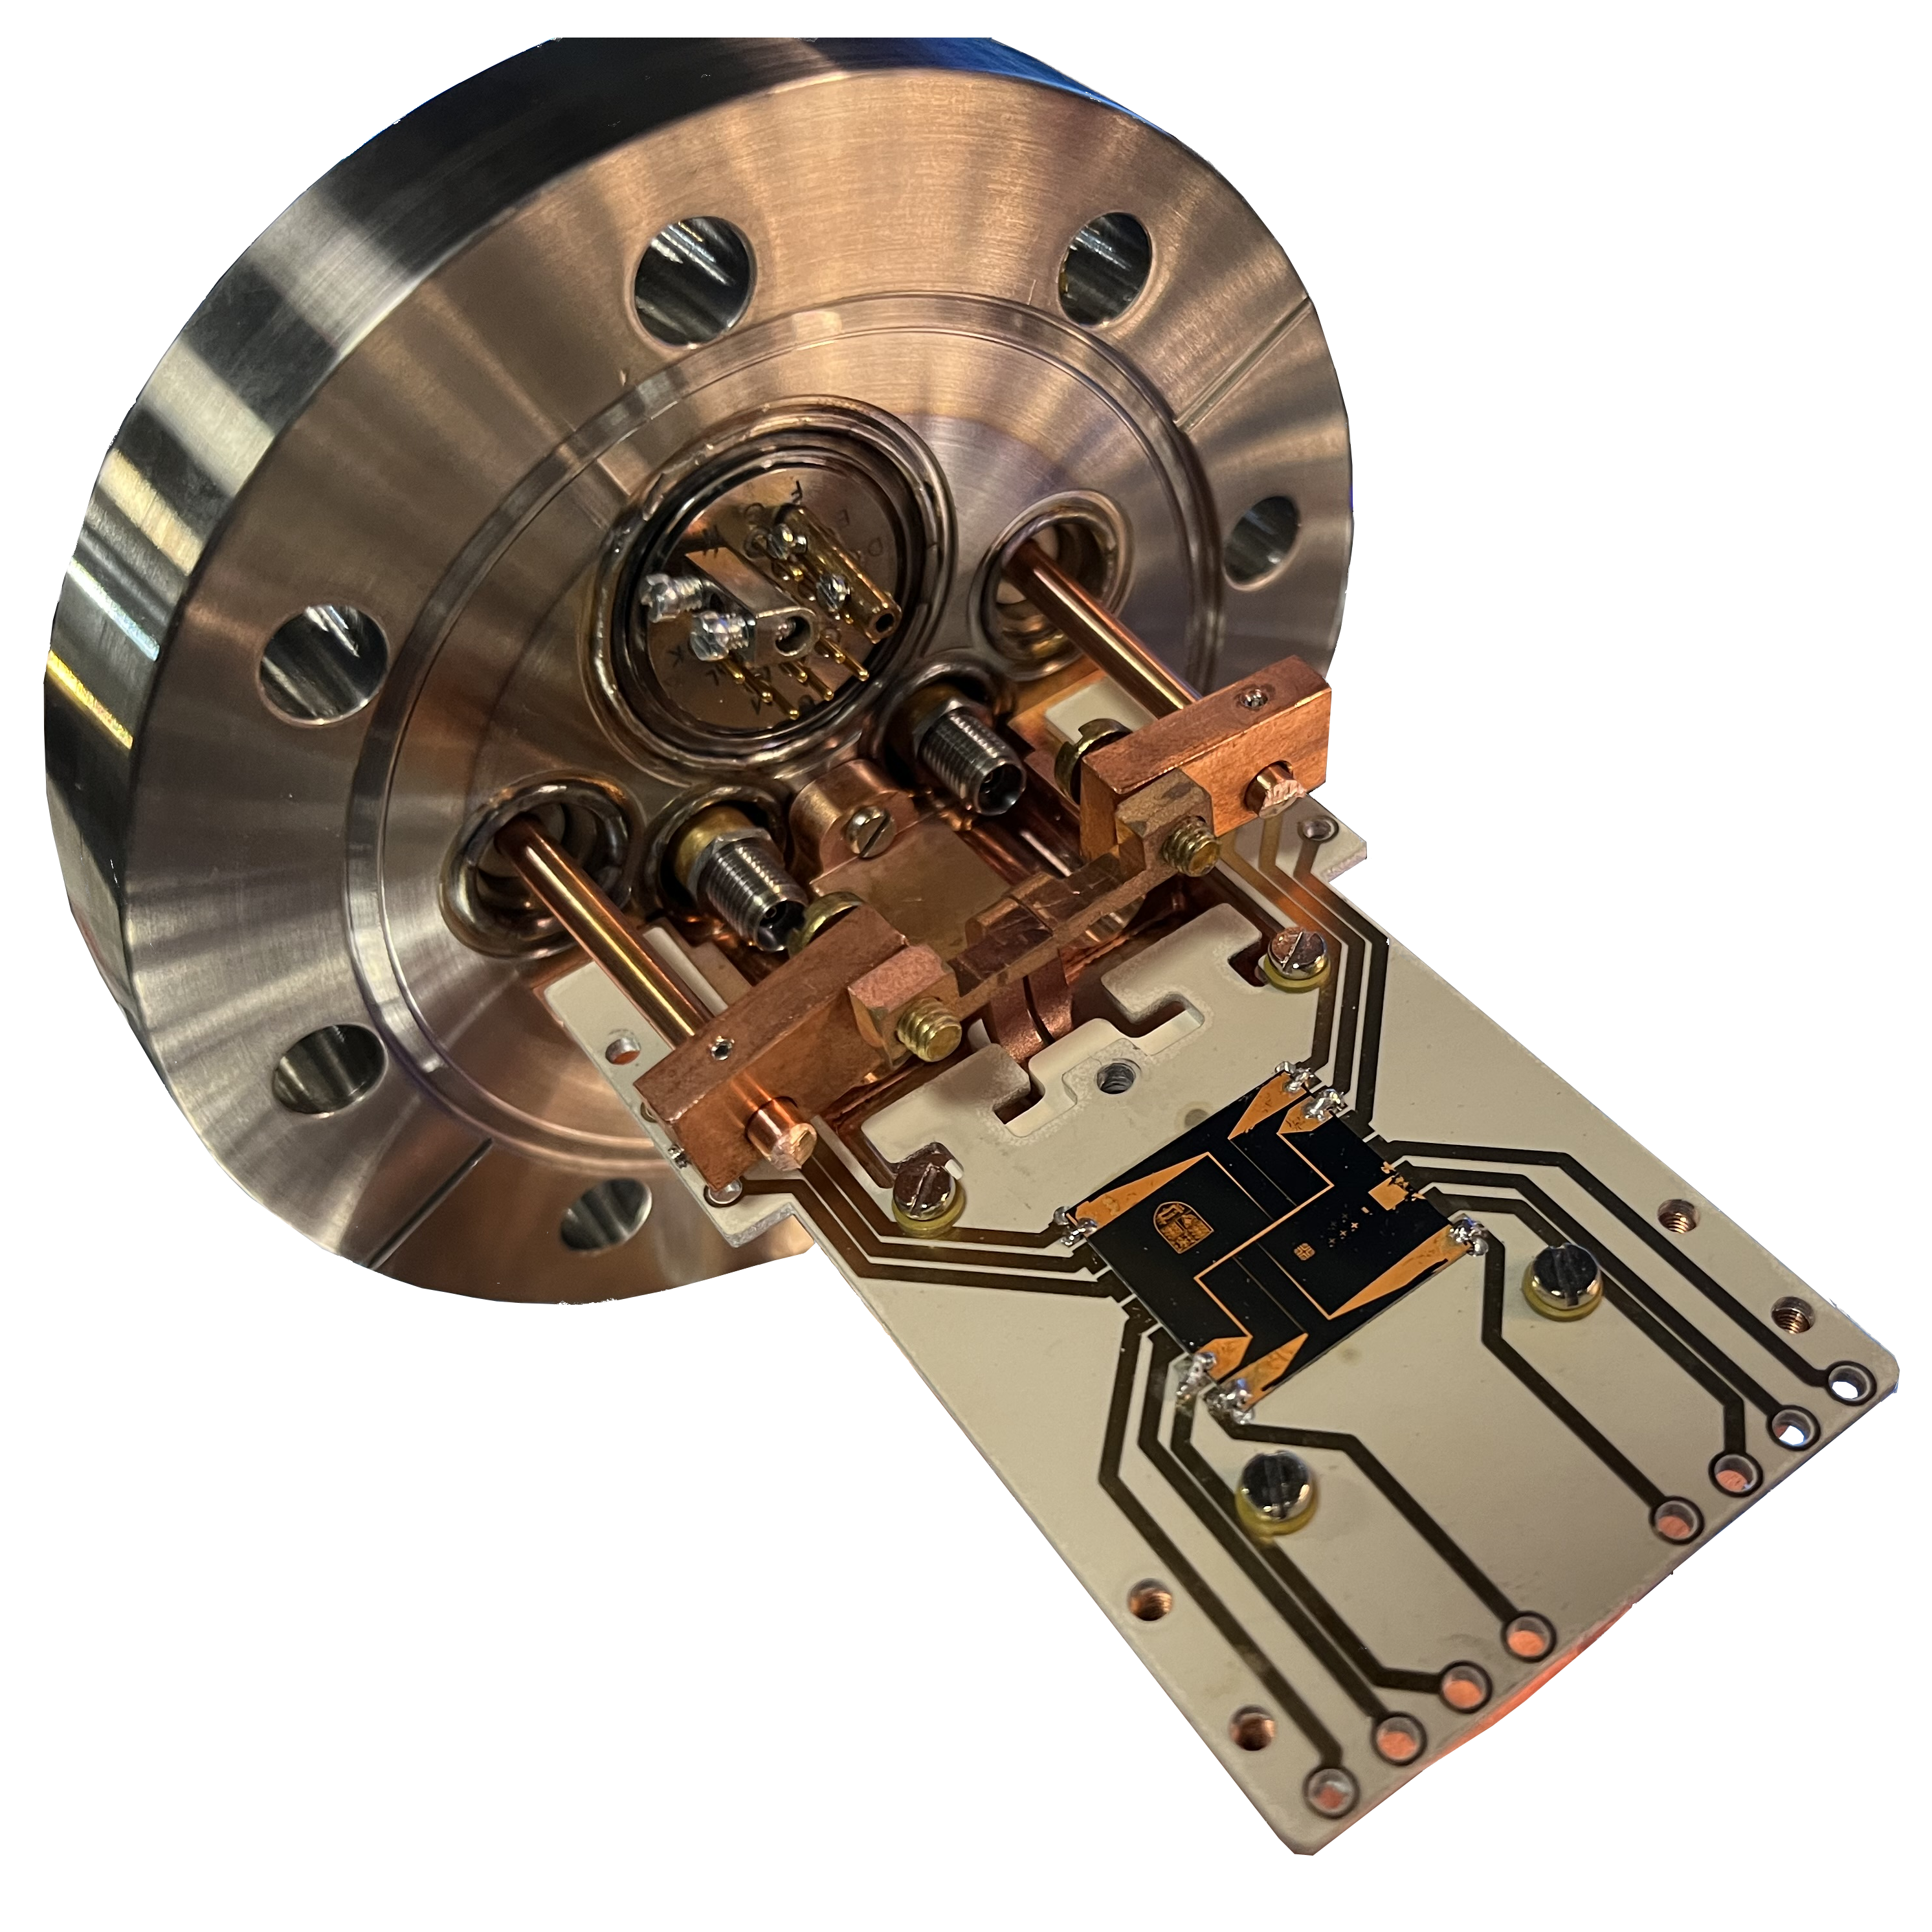
\includegraphics[width=\textwidth]{figs/chip_pic_crop.png}
    \caption{}
  \end{subfigure}
  \hspace{1cm}
  \begin{subfigure}[b]{0.45\textwidth}
    \centering
    %\includegraphics[width=\textwidth]{figs/chip_present2.pdf}
    \begin{overpic}[abs, width=\textwidth]{figs/chip_present4.pdf}
      \put(10, 160){\small (i)}
      \put(60, 160){\small(ii)}
      \put(175, 60){\small(iv)}
      \put(110, 137){\small(iii)}
      \put(70, 90){\small \SI{20}{\micro\meter}}
      \put(112, 93){\small\SI{10}{\micro\meter}}
      \put(8, 42){\small $\mathrm{Z_0}$}
      \put(8, 10){\small $\mathrm{Z_1}$}
      \put(8, 200){\small $\mathrm{Z_2}$}
    \end{overpic}
    \caption{}
  \end{subfigure}
  \caption{
    In (a) we have the chip assembly fully constructed, with a view of the
    aluminium-core PCB (subchip) for current delivery. Note also the polyimide
    bushings to electrically isolate the retaining screws from the surface. The
    microwave feedthroughs remain disconnected. In (b) we show a schematic of
    the chip features, with the scaling exaggerated for visibility. The three
    overlapping Z-wires are shown and labeled. The gaps between the wires are
    highlighted.
    %
    Toward the left (i) is the
    electroplating connection pad and various features used for
    characterisation (ii). On Z2 it is possible to see several small pads used
    as anchors, to secure the thin wire to the substrate.  The axis of the
    $\mathrm{Z1}$ wire is labeled for reference (iii) and the other wires are
    similar. All of the above features  will be discussed further in
    chapter~\ref{fab}. The crest of Imperial College London (iv) is also
    included.}
  \label{design:fig:chipexperiment}
\end{figure}

% TODO Check what these equations that I use actually are and where they go. I
% think the current wording might basically be the same equation twice...
The first stage of the magnetic transfer is to take the molecules from the MTT
to the large U-wire embedded in the heat sink.  The idea is to use this as a
deep, macroscopic trap that is well-aligned with the chip by virtue of being
built into the assembly, and can be easily aligned with the MTT, similarly to
other experiments such as \inlineref{Ott2001}.  Since it is under the chip, it
will of course be further from the molecule cloud than the other wires, hence
more current will be required to create a deep trap (as per
equations~\ref{intro:eq:trapbias} and~\ref{intro:eq:trapdepth}). The current is
limited to \SI{100}{\ampere} by the vacuum feedthroughs, allowing for a trap of
depth around \SI{2}{\milli\kelvin} by equation \cm{ref. earlier chapter}.

Once loaded into the U-trap, the molecules will be transferred through the
Z-wire traps on the chip. Each Z-wire should be sufficiently
large to maintain the currents required to form a trap at height $z$ below the
trap, whilst having a width and height  $w, h \ll z$ so that that the current
is highly localised compared to the cloud size.  This follows the widely-made
assumption in the literature that the trapping currents are carried by wires
which are infinitesimally small compared to the length scale of the trap
~\cite{2011Ac}.

In the case of the first Z-wire, the molecules are still \SI{3}{\milli\meter}
away from the trapping wire. If we demand a trap depth of
$k_B\times\SI{1}{\milli\kelvin}$, then we will require a trapping current of
\SI{30}{\ampere} to form a trap of this depth.  We will discuss in
chapter~\ref{fab} that the maximum wire height that can reliably be fabricated
is \SI{5}{\micro\meter}, and we expect that the wires will be able to carry a
maximum current density of \SI{6E10}{\ampere\per\meter\squared}, as was found
for a similar chip design in \inlineref{Treutlein2008}. The Z-wire will
therefore have a width $w=\SI{200}{\micro\meter}$. Other wire parameters are
shown in \mytableref{design:table:wires}.

The axial length of the wires also decreases to gradually reduce the size of
the trapped cloud in the $x$ direction. An exaggerated schematic of the wire
layout is shown in \myfigref{design:fig:chipexperiment} and further details are
outlined in \mytableref{design:table:wires}. All wires have been designed to
carry twice the current that is required in the loading scheme, so that there
is sufficient headroom for further experiments, and to reduce risk of
accidental damage to the chip during normal operation.

% TODO Maybe need more detail here
\begin{table}
  \centering
\begin{tabular}{lrrrrr}
  Name & Axis length (\si{\milli\meter}) & Width (\si{\micro\meter})& $I_\text{max}$ & Trap height (\si{\micro\meter}) \\
 \hline
  U & 16 & N/A& 100 & 3000\\
  $\mathrm{Z0}$ & 12 & 200& 60& $3000\rightarrow1000$ \\
  $\mathrm{Z1}$ &  6 & 20& 6& $1000\rightarrow100$ \\
  $\mathrm{Z2}$ &  2 & 2& 0.6& $100\rightarrow10$ \\
 \hline
\end{tabular}
  \caption{Details on the wire dimensions, maximum current, and desired
  trapping heights. The wire design is shown in
  \mysubfigref{design:fig:chipexperiment}{c}. Note that the U-wire current is
  limited by vacuum feedthroughs and not by the maximum current calculated by
  the wire dimensions.  The maximum currents have been designed for use at only
  50\% of their potential maximum ($I_\text{max}$).
  }
  \label{design:table:wires}
\end{table}

Each Z-trap will begin trapping at one height before the bias field is
increased to bring the trap centre closer to the surface (as per
% TODO back to link
%\myeqref{intro:eq:trapbias}
\cm{reference eqn. $B = \mu_0 I / (2\pi h)$}
).  To distinguish between the two trap stages for
each wire, we label them $\mathrm{ZX_i}$ for the initial (higher) trap and
$\mathrm{ZX_f}$ for the final (lower) trap, with $\mathrm{ZX}$ corresponding to
the wire labels in \mytableref{design:table:wires}.

In order to incorporate microwave guides onto the chip. This can be
accomplished by adding an insulating layer on top of the wires, on to which we
can fabricate coplanar waveguides~\cite{1127105}. The flange has been designed
with microwave feedthroughs, so that microwaves can be launched onto the
subchip and carried to the chip via coplanar waveguides \cm{to be discussed in
a later chapter}.

Having broadly outlined the experiment, the rest of this chapter will justify
the design of the trapping wires by means of simulation and analysis
of the trapping potentials.

\section{Motion of molecules in a trap}
\label{design:motion}

% TODO Is the Bohr magneton introduced above?
% TODO Do I introduce this ket notation above?
% TODO Maybe this is actually better in the intro when I will talk about
% weak-field seekers, etc.
We can assume that the motion of the molecules in the trap is classical. They
move in the potential $V(t, \mathbf{q}) = \mu B(t, \mathbf{q})$, where
$\mu\approx\mu_B$ is the magnetic dipole moment of the molecule in the
$\ket{1,0,-1}$ state.  The motion of any one particle is described by Hamilton's
equations,~\cite{Lichtenberg1969}
%
\begin{align}
  \label{design:eq:hamilton}
  \dot{\mathbf{q}} =  \frac{\partial H}{\partial \mathbf{p}} &&
  \dot{\mathbf{p}} = -\frac{\partial H}{\partial \mathbf{q}},
\end{align}
%
where $H$ is the classical Hamiltonian of the system
\begin{equation}
  %
  H(t, \mathbf{q}, \mathbf{p}) = \frac{\mathbf{p}^2}{2m} + V(t, \mathbf{q}).
\end{equation}
For now we neglect the time dependence of the potential, so that $V(t,
\mathbf{q}) = V(\mathbf{q})$.

Solving Hamilton's equations tells us the position and momentum of a single
particle. Taken together these two vectors describe a point in a six
dimensional phase-space of position and momentum.
%
For an ensemble of particles we often consider the envelope of the region they
occupy, calling this space the phase-space volume of the ensemble. This is a
powerful tool, since calculating the trajectory of particles on the boundary of
this region is often sufficient to describe the behaviour of the whole
ensemble. This technique is commonly used in particle trapping, and especially
when considering the behaviour of beams of particles, where a four-dimensional
phase-space is used \cite{Hand1998, Lichtenberg1969}.

It is helpful for us to write the phase-space volume $V$ in terms of the
spatial volume occupied by the ensemble ($V_\text{space}$) and its temperature.
The length-scale for a monatomic gas of temperature $T$ is the thermal de
Broglie wavelength~\cite{blundell2}
%
\begin{equation}
  \lambda_\text{dB}(T) = \frac{h}{\sqrt{2 \pi m k_B T}}.
\end{equation}
%
Hence the unitless phase-space volume is
%
\begin{equation}
  V = V_\text{space} \lambda_\text{dB}^{-3}(T).
\end{equation}
%
It is also useful to define a unitless phase-space
density~\cite{PhysRevA.52.1423}
%
\begin{equation}
  \rho = \frac{N}{V} = \frac{N \lambda_\text{dB}^3}{V_\text{space}}.
\end{equation}
%
For a given cloud with phase-space density $\rho$, trap with volume
$V_\text{trap}$ and depth $T_\text{depth}$,
the maximum possible number of particles that can be trapped is $\rho
V_\text{trap}/\lambda_\text{dB}^3(T_\text{depth})$.

A second powerful tool for determining the motion of the particles is
Liouville's theorem~\cite{Landau1982, Hand1998} states that the phase-space
volume is a conserved quantity, as long as the trapping potential is
consevative. This means that the phase-space density of a trapped molecular
cloud cannot be increased without application of some velocity-dependent
damping, such as an optical molasses~\cite{Metcalf1999}. The impact of this for
the chip is that the phase-space density of the cloud at the point of loading
onto the chip determines the maximum number of molecules that can be trapped in
the final trap.

If we do not introduce any further cooling steps, then the number of molecules
we are able to trap in the final trap will be
%
\begin{equation}
  N_\text{final} = \frac{\rho_\text{\CaF{}}V_\text{trap}}
  {\lambda_\text{trap}^3} = \frac{\rho_\text{\CaF{}} V_\text{trap}(2 \pi m_\text{CaF} k_B
  T_\text{trap})^\frac{3}{2}}{h^3}
  \label{design:eq:psd_N}
\end{equation}
%
where $\rho_\text{\CaF{}} = 3.4\times10^{-12}$ is the phase-space density of
the \CaF{} cloud after cooling in the blue-detuned molasses~\cite{Truppe2017},
$V_\text{trap}\sim(\SI{10}{\micro\meter})^3$ and
$T_\text{trap}=\SI{4}{\kelvin}$. The \CaF{} mass is
$m_\text{\CaF{}}=\SI{9.79E-26}{\kilogram}$. The trap depth used here is for the
smallest trap operating at \SI{3}{\ampere}, and can be calculated using
equation~\ref{intro:eq:trapdepth}. We therefore have
%
\begin{equation}
  N_\text{final} \lesssim 2000
\end{equation}
%
as an upper bound for the number of molecules trapped in the final trap. To
reiterate, this assumes that the entire trap is full, and no excess molecules
have been lost during loading. We will see below that this will not be the
case. A more realistic number of molecules to be trapped can be found by using
two key tools: analysis of the phase-space acceptance of the traps, and direct
trajectory simulation of the cloud.

\subsection{Phase-space acceptance}

% TODO I think it's OK to refer to depths in terms of temperature, but must be
% consistent!
For a particle to be trapped, it is obvious that it must occupy some spatial
region that is within the trapping potential and it must not have sufficient
energy to escape from said potential. In other words, the Hamiltonian of the
particle $H(\mathbf{q}, \mathbf{p})$ must be less than the trap depth
$T_\text{depth}$.  This relation defines a region of phase-space that we call
the acceptance. Any particles within this region will not have sufficient
energy to escape, and so will remain trapped under classical motion unless
externally influenced (ignoring for example any collisions, decays, Majorana
losses, etc.)~\cite{Lichtenberg1969}.

As an example consider the one-dimensional case of a harmonic trap found in 
\inlineref{Crompvoets2005}
%
\begin{equation}
  V(z) = \begin{cases}
    0 & |z| > l \\
    -\frac{1}{2}m\omega^2 z^2 & |z| \leq l.
  \end{cases}
\end{equation}
%
Here, any particle which starts with a position $l \leq z \leq l$ will be
trapped, so long as its velocity is not sufficiently large that it will escape
into the $|z|> l$ region. To reach $z=l$ from an initial position $z_0$, the
particle must have kinetic energy of at least
%
\begin{equation}
  \frac{1}{2}mv_0^2 = \frac{1}{2}m\omega^2(l^2 - z_0^2)
\end{equation}
%
where $v_0$ is the initial velocity. It is now clear that a particle is trapped
on the condition that
%
\begin{equation}
  (v_0/\omega)^2 + x_0^2 < l^2
\end{equation}
%
which defines an ellipse in phase-space.

% Note that in the simulation I have omega = 1, so taking omega -> 1000 means
% that we end up with the nice circle with v in m/s. The consequence is that
% the simulation ends up lasting 1.2ms rather than 1.2s

% TODO Want to be able to ref. multiple subfigs?
This trapping condition can be verified by simulation, as is shown in
\myfigref{design:fig:psaeg} (a) and (d), where the trap has been simulated for $m =
1$, $\omega = \SI[parse-numbers=false]{10^3}{\radian\per\second}$ and $l
=\SI{1}{\milli\meter}$. We initialise 2000 particles uniformly distributed with
$|z_0| < \SI{0.2}{\milli\meter}$ and $|v_0|< \SI{1.5}{\meter\per\second}$,
their trajectories are computed for \SI{1.2}{\milli\second} by the methods
described in the next section. The boundary of the acceptance, called the
separatrix is shown in black. All particles that are initialised inside the
acceptance remain trapped and evolve through time in the usual way for a
harmonic potential.  Particles initialised outside the acceptance are rejected
and lost.

It is also instructive to consider anharmonic potentials, for example
%
\begin{equation}
  V(z) = -V_0\cos(\omega z)
\end{equation}
%
which is also presented in \myfigref{design:fig:psaeg}, using the same
parameters as for the previous potential. We again see that particles with
sufficiently low energy in the trapping region remain trapped, however in this
case the anharmonicity of the trap results in the particle cloud spiralling
outwards, undergoing an effective increase in the phase-space density.

Finally, it is useful to consider the phase-space acceptance of a wire trap.
For simplicity we begin by considering only the acceptance in the $z$ direction
(perpendicular to the chip surface). Acceptance of a Z-wire with an axis of
\SI{20}{\milli\meter}, current of \SI{40}{\ampere} and a trapping height of
\SI{3}{\milli\meter}. The particles are initialised such that they have no
motion in the $x$ and $y$ directions, and the trajectories are simulated for
\SI{200}{\milli\second}. The distributions as initialised and at the end of the
simulations so that $0.1 < z/\si{\milli\meter} < 1.5$ and
$|v_z|<\SI{0.2}{\meter\per\second}$ as shown in \myfigref{design:fig:psaeg}.
The accepted molecules (blue) are once again those that start inside the
separatrix. There are also metastable molecules (orange) which remain outside
the acceptance but stay nearby the trap. These are molecules with nearly
sufficient energy to escape the trap, but may take some time to do so.

\begin{figure}[htb]
  \centering
  \import{figs/simsThesis/}{psa_1D.pgf}
  \caption{
    The phase-space acceptance for harmonic (a, d), anharmonic (b, e) and
    Z-wire trap (c, e) are shown. The top row shows the initial positions of
    the particles: those that are accepted by the trap are shaded blue,
    particles that are lost are shaded red, and metastable particles in orange.
    The energy contour of the trap depth is also shown. The end state of the
    simulation is shown in the lower row. Note the filamentation effect in (e)
    and (f), where the effective phase-space density of the particles increases
    as they explore regions that are energetically accessible. The harmonic and
    anharmonic examples are inspired by discussion in
    \inlineref{Crompvoets2005}.
  }
  \label{design:fig:psaeg}
\end{figure}


Note that if we were to turn off these traps then the particles would be
emitted directly into the phase-space volume shown on the bottom row of
\myfigref{design:fig:psaeg}. If we were to try to recapture them then the new
trap would have to be positioned so that the particles were inside its
acceptance. We call the occupied area of phase-space at the end of the trapping
period the trap's phase-space emittance.

It is therefore clear that a particle that is stored in one trap can be moved
into another if its position in phase space is inside the separatrix of the new
trap. Hence we design the trapping potentials such that the emission of one
trap overlaps with the acceptance of the next one in the loading sequence. This
is similar to the mode-matching of potentials described in, for example,
\inlineref{2011Ac}. We will see below that the matching of trap acceptances
does indeed allow for reliable loading of the traps

% TODO Check this strong statement on L's theorem
While this applies to a rapid switching off and on of trapping potentials, we
note that it is possible to adiabatically transform potentials in such a way
that the phase-space density of the ensemble remains unchanged. This can be
achieved because the Liouville theorem also holds for time-dependent
Hamiltonians, as long as the potential remains conservative
throughout~\cite{Hand1998, Lichtenberg1969}. Hence a cloud of trapped particles
can be translated, for example in the transport coils, or towards the surface
of the chip as will be discussed in section~\ref{design:adiabatic}.

% TODO Also I'm not sure about this subsection's location, maybe it should go
% up but leaving it here for the time being.
\subsection{Simulating the motion}
\label{design:motion:simmethods}

The motion of a particle can be simulated by numerically solving
\myeqref{design:eq:hamilton}, which we do using Python~\cite{python} and the
symplectic Euler method~\cite{Hairer2015, doi:10.1119/1.2034523} provided by
the Desolver package~\cite{desolver}. Symplectic methods are powerful tools
for numerically solving Hamiltonian systems whilst conserving energy and
momentum.
%
We are able to simulate any arbitrary potential, such as those already
discussed in the previous section, but it is useful to consider a more
realistic potential given by the sum of the magnetic and gravitational
potentials,
%
\begin{equation}
  V(t, \mathbf{q}) = V_\text{mag} + mg(z_0-z)
\end{equation}
where $g=\SI{9.8}{\meter\per\second\squared}$ is the acceleration due to
gravity, and $z_0$ is an arbitrary point chosen to be the zero of the
gravitational potential. The actual value chosen does not matter as it
constitutes only a linear offset in the entire potential, we normally present
the potentials with $z_0$ chosen such that the trap minimum is zero.
%
The Van der Waals attraction between the chip and the molecules is neglected,
since the molecules will (by design) never be close enough to the chip for this
force to be significant.

% TODO Move this to theory?
When simulating the motion of the particles in a quadrupole coil trap (such as
the MTT), the magnetic field is assumed to be an idea quadrupole, so
%
\begin{equation}
  \mathbf{B}(x, y, z) = B'\begin{pmatrix} -x/2 \\ -y/2 \\ z \end{pmatrix}
\end{equation}
where $B'$ is the field gradient. \cm{This eqn. will probably end up in an earlier
chapter.}

The magnetic potentials of the wire traps are calculated by considering the
traps to be formed of segments of straight wires, each producing a magnetic
field $\mathbf{B}_\text{seg}^{(i)}$, and the bias field
$\mathbf{B}_\text{bias}(t)$.  The total field is the sum of contributions from
the set of all segments ($S$), and the bias. The potential is therefore
%
\begin{equation} V\text{mag}(t, \mathbf{q}) = \mu B (t, \mathbf{q}) = \mu
\left| \sum_{i\in S} \mathbf{B}_\text{seg}^{(i)}(t, \mathbf{q}) +
\mathbf{B}_\text{bias}(t)\right|.  \end{equation}
%
Where the field of each wire segment is~\cite{Griffiths2017}
%
\begin{equation} \mathbf{B}_\text{seg}(t, \mathbf{q}) = \frac{\mu_0 I(t)}{4\pi
s_\text{seg}(\mathbf{q})} (\sin(\theta_2)  -
\sin(\theta_1))\hat{\mathbf{\phi}}. \label{design:eq:segmentfield}
\end{equation}
%
Here $s_\text{seg}(\mathbf{q})$ represents the shortest distance between the
point $\mathbf{q}$ and the line that runs through the segment off to infinity
in each direction. We also have the unit vector $\hat{\mathbf{\phi}} =
\mathbf{I}\times\mathbf{q}/(qI)$.

\begin{figure}[h]
\centering
  \begin{tikzpicture}
    % Def coords
    \coordinate (O) at (0, 0);
    \coordinate (L) at (-3, 0);
    \coordinate (R) at (3, 0);
    \coordinate (Q) at (-4, 4);
    % Draw lines
    \draw[line width=0.75mm, ->] (L) -- (R);
    \draw (L) -- (Q);
    \draw (R) -- (Q);
    \draw[<->, densely dotted,shorten >=.5mm,shorten <=.8mm] (Q) -- (-4, 0);
    % Draw line parallel to wire
    \draw[-, dashed] (-5, 0) -- (L);
    \draw[-, dashed] (R) -- (5, 0);
    % Draw dot at Q
    \node at (Q)[circle,fill,inner sep=.5mm]{};
    % Draw angels
    \draw pic[draw,angle radius=1cm,"$\theta_1$" shift={(7mm,2mm)}] {angle=R--L--Q};
    \draw pic[draw,angle radius=1cm,"$\theta_2$" shift={(-7mm,2mm)}] {angle=Q--R--L};
    % Label
    \node[shift={(4mm,0)}] at (Q) {$\mathbf{q}$};
    \node[shift={(2mm, 4mm)}] at (R) {$I$};
    \node[fill=white] at (-5.0, 1.8) {$s_\text{seg}(\mathbf{q})$};
  \end{tikzpicture}
  \caption{Geometry of a wire segment (bold) carrying current $I$, whose field
  can be calculated using \myeqref{design:eq:segmentfield}. The dotted line
  shows $s_\text{seg}(\mathbf{q})$, the shortest distance from the point at
  which the field is calculated ($\mathbf{q}$) to the line parallel with the
  wire (dashed line).
  }
  \label{design:fig:wiresegment}
\end{figure}

%In the case of that we are exchanging between
%two potentials, the segments of both traps are included in the summation, with
%the currents becoming functions of time, and similar for exchange between a
%quadrupole and a wire trap, with the quadrupole gradient being a function of
%time.

\subsection{Simulation initialisation}
\label{design:sim:init}

For all the simulations described below, we begin with a cloud of molecules in
a magnetic quadrupole trap. We use the following initialisation procedure so
that the distribution of our molecules matches that which we expect in the
experiment. 
%
The simulation begins with a cloud of $N$ molecules whose positions are normally distributed
in all three spatial dimensions with a standard deviation of $\sigma_i$
(typically $\sigma_i = \SI{1}{\milli\meter}$). Similarly the velocity components
are normally distributed with a standard deviation of $\sigma_{v_i}$ (typically
\SI{40}{\milli\meter\per\second}, corresponding to a temperature of
\SI{5}{\micro\kelvin}). 

The cloud is initialised in a quadrupole trap with gradient
\SI{10}{\gauss\per\centi\meter}. They are held for \SI{50}{\milli\second}
before the gradient is linearly ramped over \SI{100}{\milli\second} to
\SI{60}{\gauss\per\meter} (the gradient used in the MTT).  The molecules are
then held for a further \SI{50}{\milli\second}, as a stabilisation time.  The
increasing trap gradient causes the molecules to compress as they would when
initially loaded into the transport coils in the MOT chamber.

% TODO I anticipate needing to put some comparison to the real data here...
\cm{Maybe I need to compare to actual data here, or put some plots of the
simulation after initialisation, but I'm not really sure. What do you think?}

\section{Adiabatic transfer between traps}
\label{design:adiabatic}

It should be obvious that if we start with molecules in one potential, then
rapidly turn that one off and turn on another, this will cause heating and
increase its size.  However, if we ramp between the traps adiabatically then
we expect the effect on the cloud size to be minimal. In order to understand
how best to load the chip trap it is important that we understand the extent
of heating in the case of rapid transfer and the timescale required to be
adiabatic.

We investigate this with a simple example: consider two ideal quadrupoles
with gradients of \SI{60}{\gauss\per\centi\meter} separated by
\SI{3}{\milli\meter} in the $x$ direction. We simulate 2000 \CaF{} molecules
using the above-described initialisation procedure, with initial $\sigma_i =
\SI{2}{\milli\meter}$ in all directions, and initial temperature
$T=\SI{50}{\micro\kelvin}$. We ramp linearly between the potentials in a time
$t_\text{ramp}$, which we vary between \SI{1}{\milli\second} and
\SI{100}{\milli\second}. The molecules are then held for a further
\SI{100}{\milli\second}. The state of the system at the end of the simulation
is shown for $t_\text{ramp}\in \{\SI{1}{\milli\second}, \SI{30}{\milli\second},
\SI{100}{\milli\second}\}$ in \myfigref{design:fig:adia3sim}, along with the
behaviour of the cloud in the \SI{100}{\milli\second} hold time. Note that as
the ramp time increases, the oscillation in cloud size, temperate and position
decreases, as we have said we expect.

\begin{figure}[p]
\centering
  \import{figs/simsThesis/}{adiabatic_3sim.pgf}
  \caption{
    Exchange between two quadrupole traps, separated by \SI{3}{\milli\meter} at
    different ramp times. The top row shows the $x$-projection of the
    phase-space distributions of the particles at the start of the simulation
    (grey) and after various ramp times (see legend) followed by a
    \SI{100}{\milli\second} hold in the displaced trap. The mean position, size and
    temperature of the cloud are shown throughout the hold time for each
    simulation. Note that for the longer ramps we observe less severe heating,
    oscillation and widening of the cloud.
  }
  \label{design:fig:adia3sim}
\end{figure}


The question then is at what point do we enter the adiabatic r\'egime?
\myfigref{design:fig:adiavary} shows the cloud width and temperature at the end
of the simulation for varying $t_\text{ramp}$. After
$t_\text{ramp}\sim\SI{50}{\milli\second}$ the reduction is minimal, and we are
strongly in the adiabatic r\'egime. This is approximately the timescale we
would expect, since the timescale for a quadrupole trap is
%
\begin{equation}
  \tau = \sqrt{\frac{2 m }{\mu_B B'}}
\end{equation}
%
\cm{this will be moved to theory and explained properly there}, so $\tau \sim
\SI{10}{\milli\second}$ for such a trap. \cm{We need $t \gg \tau$ to be
adiabatic.}

\begin{figure}[t!]
\centering
  \import{figs/simsThesis/}{adiabatic_varyramps.pgf}
  \caption{
    The final temperature and size of particle clouds transferred between
    offset quadrupole traps at various ramp times. Note that the large
    oscillations in width that occur for short ramp times (see
    \myfigref{design:fig:adia3sim}) can result in the instantaneous width of
    the cloud being small, such as in the shorter ramp times here.
  }
  \label{design:fig:adiavary}
\end{figure}

% TODO I do have some stuff about rapid vs. adiabatic transfer between z-traps,
% but I think it is unnecessary.

\section{Trajectory simulation of the initial loading stages}

In this section we will present simulations of loading molecules from the MTT
into the on-chip Z-wire traps. 
This demonstrates
the two main types of transitions in the loading process: handovers between
traps, and compression within a single trap. The timing of the simulation do
not exactly reflect those that will be used in practice and long holding periods
have been inserted between ramps to better illustrate the cause of particle
loss. It is useful to perform direct trajectory simulations as opposed to
simple analysis of the phase-space emittance and acceptance, since (as we will
see later) brief lowering of trap depth during trap handovers can induce
additional loss of particles.

We will consider the handover in four stages: the particle initialisation, which
was already discussed in section~\ref{design:sim:init}; followed by the
handover from the MTT to the U-wire; then the U-wire to $\mathrm{Z0_i}$.
Finally we will simulate the compression in the Z-wire trap from
$\mathrm{Z0_i}$ to $\mathrm{Z0_f}$. A full summary of the changing parameters
throughout the simulations is given at the end of the section, see especially
\myfigref{design:fig:simsum}.

\subsection{MTT - U transfer}
\label{design:sim:trans_U}

The cloud is initialised by the usual procedure, with $\sigma_i =
\SI{1}{\milli\meter}$ and $T=\SI{50}{\micro\kelvin}$, corresponding to the
typical cloud sizes and temperatures we measure in the tweezer chamber after
transport. Over \SI{100}{\milli\second} the field from the coils is linearly
redued to zero and the U-wire current is ramped up to its maximum value of
\SI{100}{\ampere}. The bias fields in the $y$ and $z$ directions (no $x$ bias
is applied) are also ramped linearly, to maintain the trap centre at a height
of \SI{3}{\milli\meter} below the chip. The state of the system before and
after the ramp is shown in \myfigref{design:fig:mttusim}.

\begin{figure}[p]
\centering
  \import{figs/simsThesis/}{mtt_u_summary.pgf}
  \caption{
    The simulation of the transfer from the MTT to the U-wire. The state of the
    system is presented at the end of the initialisation procedure (blue) when
    the trapping potential is that of the MTT, and after ramping to the U-trap
    (red). The phase-space distributions are shown in the $z$-$v_z$ plane in
    (a) and (b), with histograms of the $z$ and $v_z$ projections in (c) and
    (e) respectively. The potentials at the start and end of the transfer are
    shown in (d). Subfigure (f) shows the temperature particle number varying
    throughout the fields are varied in the times that are shaded grey (c.f.
    \myfigref{design:fig:simsum}). \cm{Comment on the results.}
  }
  \label{design:fig:mttusim}
\end{figure}

The phase-space distribution in the $z$-$v_z$ projection is shown for the start
(\mysubfigref{design:fig:mttusim}{a}) and end
(\mysubfigref{design:fig:mttusim}{b}) of the simulation. Note that there is
little change to the velocity distribution, but in position the particles shift
to occupy the positive $z$ direction, where the potential is less steep.

Looking at the change in the particle number throughout the ramp
(\mysubfigref{design:fig:mttusim}{f}) it is clear that there is some loss
during the ramp (shaded grey region of the figure). We would naively expect
there to be no loss during this transfer, since the final trap depth is larger
than the temperature of the cloud, and there is good mode-matching of the two
potentials. To see why this loss occurs, we  look at the evolution in
phase-space for each projection throughout the ramp, as shown in
\myfigref{design:fig:mttudetail}.

\begin{figure}[htp]
\centering
  \begin{tabular}{c}
  \import{figs/simsThesis/}{mtt_u_detail_x.pgf} \\
  \import{figs/simsThesis/}{mtt_u_detail_y.pgf} \\
  \import{figs/simsThesis/}{mtt_u_detail_z.pgf}
  \end{tabular}
  \caption{
    Each pair of rows shows the phase-space plots for the MTT to U-trap
    handover simulation in the $q_i$-$v_i$ plane, along with the cut-through of
    the potential through the trap centre along $q_i$ at various times. This
    supplements the simulation summary shown in \myfigref{design:fig:mttusim}.
    The superposition of the quadrupole and U-traps briefly causes a lowering
    of the trapping potential, as can be seen at \SI{75}{\milli\second}. These
    reductions can occur when moving between different types of traps, such as
    from the coil-based to wire trap, or from a quadrupole to Ioffe-Pritchard
    trap. Care must be taken in such cases to ensure the potential remains
    conservative and sufficiently deep throughout the handover.
}
  \label{design:fig:mttudetail}
\end{figure}

% TODO Check this, what's the temp at these leaks?
At $t=\SI{175}{\milli\second}$ there is a noticeable decrease in the trapping
depth in the $-y$ and $+z$ directions. This is the cause of the particle leak,
and occurs due to the due to the superposition of the two fields causing an
overall decrease in the trap depth in the $x$ and $y$ directions. This only
occurs for a brief period during the ramp (lasting approximately
\SI{40}{\milli\second}).  Hence some of the more energetic particles are lost,
as can be seen in the figure.

\subsection{U - Z transfer}
\label{design:sim:U_to_Z0i}

The next stage of loading is the U to $\mathrm{Z0_i}$ handover. We simulate
this process as a continuation of the MTT-U transfer. 
The $z$
bias field is switched off instantaneously and the Z-wire current is then linearly
ramped on over \SI{100}{\milli\second} to \SI{30}{\ampere}. The bias fields are
linearly ramped to maintain the trap height at \SI{3}{\milli\meter}.
%
The simulation is presented in \myfigref{design:fig:uzsim}. We see that there
is once again a loss of particles, which we can attribute to a similar lowering
of trap depth during the handover as was seen for the MTT-U handover.  Other
than this, we see that there is minimal change in the particle distribution in
space and velocity.

% TODO Fix bias field in z not going off rapidly
\begin{figure}[p]
\centering
  \import{figs/simsThesis/}{u_z_summary.pgf}
  \caption{
    The U-trap to Z-trap handover is summarised, with subfigures and colours as
    in \mysubfigref{design:fig:mttusim}. Here we again see loss effects similar
    to those seen for the MTT to U-trap handover, with a decrease in trap depth
    which we attribute to changing from a quadrupole trap to a Ioffe-Pritchard
    trap.
  }
  \label{design:fig:uzsim}
\end{figure}

\subsection{Z compression}

The final stage of the loading procedure is a linear ramp of the trap height
from \SI{3}{\milli\meter} below the chip surface to \SI{1}{\milli\meter} below.
Here only the $y$ bias field is changed so  that the trap depth
increases and the cloud is compressed, providing good localisation of the
molecules. Ramping the height linearly requires the bias to change as a
function of time so that $B_{\text{bias}, y} \propto t^{-1}$.

As can be seen in \myfigref{design:fig:zsim}, there is particle loss,
although much of this is due to particles that had already left the trapping
region in the previous ramp, note that in subfigure~(f) the particle number is
decreasing before the ramp begins. The other major effect of the ramp is
heating, which occurs due to the spatial compression and conservation of
phase-space density.
%
The transfer of the cloud towards the chip surface is succesful, as can be seen
in \mysubfigref{design:fig:zsim}{e}, the particles are highly localised around
the new trap minimum at $z=\SI{1}{\milli\meter}$.

\begin{figure}[p]
\centering
  \import{figs/simsThesis/}{z_summary.pgf}
  \caption{
    The Z-trap compression simulation is summarised, with subfigures and colours as
    in \mysubfigref{design:fig:mttusim}. The particle loss before the ramp
    begins is due to effects from the U-Z handover. We experience minimal
    particle loss in the compression, and the depth of the trap increases
    significantly, so that despire the heating of the cloud there is good
    localisation close to the surface.
  }
  \label{design:fig:uzsim}
\end{figure}}
  \label{design:fig:zsim}
\end{figure}

\subsection{Summary of the simulation}

The entire simulation from MTT to $\mathrm{Z0_f}$ is summarised in
\myfigref{design:fig:simsum}. For each stage: initialisation (a), MTT-U
transfer (b), U-Z transfer (c) and Z compression (d) the particle number is
shown. The total temperature and cloud width are also given for the particles
that remain in the trap at the end of the simulation. The profile of parameters
that are changed for each ramp are also shown. 


\begin{figure}[p]
\centering
  \import{figs/simsThesis/}{total_summary.pgf}
  \caption{
    Details for each stage of the simulation in turn. Column (a) shows the
    initialisation procedure. Column (b) shows the ramp from the MTT to U-wire,
    with the ramp duration shaded grey. During the ramp handover there is some
    expansion of the cloud, which causes oscillations in the width that can be
    seen continuing on into the next phase. In column (c) we have the U-Z
    handover and the $z$ bias field is switched off. Finally in column (d) is the
    compression in the Z-trap, note in particular the increase in cloud
    temperature as the width decreases. The lower two rows show the parameters
    of the simulation that are changed to alter the trapping potentials.
  }
  \label{design:fig:simsum}
\end{figure}

The simulation shows that the loading of the initial chip trap can bring in
approximately 60\% of the initial cloud. We assumed an initial temperature of
\SI{50}{\micro\kelvin}, however refining the transport process could allow us
to load clouds of lower temperatures, which could mean that a higher loading
efficiency is possible. It may also be possible to implement some cooling in
the chip chamber to reduce this temperature, but we are restricted by the
limited optical access.
%
Heating in the trap is largely due to the compression in the final stage. This
is inevitable, but does not cause any problems, since the trap depth
increases for traps closer to the surface, and the molecules are
well contained.

The trajectory simulation discussed in this section is instructive, since it
tells us something about the handovers between different types of traps. Notice
that the largest source of particle loss is when converting from the quadrupole
U-trap to the Ioffe-Pritchard Z-trap. Here it is not sufficient to look just at
the phase-space emittance and aceeptance at the end of each traps, but we must
investigate the potential across the ramp, since a brief lowering of the
potential can induce enormous loss. Fortunately this is not an issue when
compressing and handing over between Z-traps, and the phase-space analysis is
sufficient for the rest of the procedure.

\section{Phase-space acceptance of remaining Z-traps}
\label{design:transferbetweenzs}

% TODO This is quite weak I think. Let's see if Mike says I should run some
% numbers, it seems kind of trivial and this chapter is already very long.
Once trapped in $\mathrm{Z0_f}$, the remaining loading stages are simply
repeated handovers to the smaller wires, with a compression stage carried out
on each wire to bring the molecules closer to the surface. This is a
well-understood and robust procedure that has been used before to load atom
chips with minimal losses~\cite{Reichel2002}. The ramps used are detailed in
table~\ref{design:table:wires}.  The timing aof the ramps could be shorter for
the Z-traps, since the timescale of motion in these traps is higher. This, as
well as the optimal shape of the ramp can be deterimined empirically.

That said, since our experiment will operate with a significantly lower phase
space density than previous experiments with atoms, it is important to ensure
that our loading procedure will not suffer from any unnecessary losses. These
compressed traps contain hotter molecules, requiring a smaller time step for
simulation. It is therefore easier to directly examine the acceptance of each
trap. We also note now that the trap gradients are sufficiently large the the
effects of gravity can be ignored.

The trap acceptances are shown in \myfigref{design:fig:phasematchinggrid},
starting with $\mathrm{Z0_f}$ in row (a). The region of the trap that we expect
to be occupied (as determined by the simulation above) is marked with a dashed
line.  This cloud of molecules will be adiabatically transferred into
$\mathrm{Z1_i}$.

Since the process is adiabatic, we can anticipate that there will be no
reduction in phase-space density. The cloud of molecules will be transferred to
$\mathrm{Z1_i}$ with negligible heating. However, the total acceptance of the
trap is less than the expected phase-space volume of the cloud, so there
will be particle loss due to spillover. The particles will undergo
fillamentation, increasing the effective phase-space density so that the
envelope of the ensemble approaches the separatrix.

Next, $\mathrm{Z1_i}$ is adiabatically compressed to $\mathrm{Z1_f}$, with the
molecules held \SI{100}{\micro\meter} from the surface. Again, this
compression is adiabatic, so we expect no change in the phase-space density.
Compression increases the trap acceptance, so there is also no loss of
particles. This is further supported by the simulated compression of
$\mathrm{Z0_i}$ to $\mathrm{Z0_f}$ discussed above. The acceptance of
$\mathrm{Z1_I}$ is shown in \mysubfigref{design:fig:phasematchinggrid}{b}, with
the expected occupation shown by the dashed line.

Finally, $\mathrm{Z2}$ is loaded and compressed in exactly the same way as
$\mathrm{Z1}$. The adiabatic handover from $\mathrm{Z1_f}$ to $\mathrm{Z2_i}$
is the final cause of particle loss (due to spillover). Then the trap is
compressed to hold the particles \SI{10}{\micro\meter} from the surface, as
shown in \mysubfigref{design:fig:phasematchinggrid}{c}.

\begin{figure}[htb]
\centering
  \begin{overpic}[page=1]{figs/sims/phase_matching_grid.pdf}
    \put(0,68){(a)}
    \put(0,44.5){(b)}
    \put(0,21){(c)}
  \end{overpic}
  \caption{
    The acceptance (solid) and expected occupation (dashed) of each Z-wire
    trap. This is calculated by finding the acceptance in the weak ($x$)
    trapping direction. Row (a) shows $\mathrm{Z0_f}$, with occupation
    determined by the above simulation. Molecules will be adiabatically
    transferred to $\mathrm{Z1_i}$, which will be fully occupied. Some
    particles will be lost due to the decrease in acceptance but this is to be
    expected, and phase-space density should not increase. In (b) we have the
    acceptance and occupation of $\mathrm{Z1_f}$ following adiabatic
    compression.  Particles will be adiabatically transferred into
    $\mathrm{Z2_i}$, resulting in similar losses to the previous step. Row (c)
    shows the final acceptance and occupation of $\mathrm{Z2_f}$.
  }
  \label{design:fig:phasematchinggrid}
\end{figure}

% TODO I don't think this makes any sense. Need to address.
Particle loss during the procedure is dominated by phase-space mismatching in
the $x$ direction. In both cases we can anticipate the loss will be
approximately a factor of two. Combined with the trajectory simulation above,
we therefore expect the final loading efficiecy to be about 15\%.

\section{Summary}

In this chapter I have presented the design of the chip experiment, starting
with the source of molecules up to the stage of confinement in a Z-trap
\SI{10}{\micro\meter} from the chip surface. I have shown that we have created
a loading procedure that will allow us to load this final trap through a series
of wire traps of decreasing size. This is justified by simulation and
phase-space analysis of the acceptance of the various trapping stages.

The design leaves scope for the addition of microwave guides on a second layer
above the trapping wires, as discussed in chapter~\ref{intro}.
